\documentclass{article} % For LaTeX2e
\usepackage{nips14submit_e}
\usepackage{times,graphicx}
%\usepackage{hyperref}
\usepackage{url}
\usepackage{amsmath}
\usepackage{amssymb}
\usepackage[small,tight]{bibhacks}
\nipsfinalcopy
%\documentstyle[nips14submit_09,times,art10]{article} % For LaTeX 2.09


\title{Sequence to Sequence Learning\\with Neural Networks}
%\title{Machine Translation with Recurrent Neural Networks}


\author{
Ilya Sutskever \\
Google\\
\texttt{ilyasu@google.com} \\
\And
Oriol Vinyals \\
Google\\
\texttt{vinyals@google.com} \\
\And
Quoc V. Le \\
Google\\
\texttt{qvl@google.com} \\
}




% The \author macro works with any number of authors. There are two commands
% used to separate the names and addresses of multiple authors: \And and \AND.
%
% Using \And between authors leaves it to \LaTeX{} to determine where to break
% the lines. Using \AND forces a linebreak at that point. So, if \LaTeX{}
% puts 3 of 4 authors names on the first line, and the last on the second
% line, try using \AND instead of \And before the third author name.

\newcommand{\fix}{\marginpar{FIX}}
\newcommand{\new}{\marginpar{NEW}}

%\nipsfinalcopy % Uncomment for camera-ready version

\begin{document}


\maketitle

\begin{abstract}

Deep Neural Networks (DNNs) are powerful models that have achieved
excellent performance on difficult learning tasks. Although DNNs work
well whenever large labeled training sets are available, 
they cannot be used to map sequences to sequences.  In this paper, we
present a general end-to-end approach to sequence learning that makes
minimal assumptions on the sequence structure. Our method uses a
multilayered Long Short-Term Memory (LSTM) to map the input sequence
to a vector of a fixed dimensionality, and then another deep LSTM to
decode the target sequence from the vector.  Our main result is that
on an English to French translation task from the WMT'14 dataset, the
translations produced by the LSTM achieve a BLEU score of 34.8 on the
entire test set, where the LSTM's BLEU score was penalized on
out-of-vocabulary words. Additionally, the LSTM did not have
difficulty on long sentences. For comparison, a phrase-based
SMT system achieves a BLEU score of 33.3 on the same dataset.  When we
used the LSTM to rerank the 1000 hypotheses produced by the
aforementioned SMT system, its BLEU score increases to 36.5, which
is close to the previous best result on this task.  The LSTM also learned sensible
phrase and sentence representations that are sensitive to word order
and are relatively invariant to the active and the passive voice.
Finally, we found that reversing the order of the words in all source
sentences (but not target sentences) improved the LSTM's performance
markedly, because doing so introduced many short term dependencies
between the source and the target sentence which made the optimization
problem easier.

\end{abstract}


\section{简介}

深度神经网络(DNN)是非常强大的机器学习模型,在诸如语音识别 \cite{hinton12,dahl12b} 和视觉对象识别 \cite{kriz12,ciresan12,lecun98,le12} 等困难问题上取得了出色的性能。DNN很强大,因为它可以在适当数量的步骤内执行任意的并行计算。强大DNN的一个令人惊讶的例子是他们只使用2个隐藏层就能够排序$N$个 \!\!\!\!\quad $N$位数的能力\cite{razborov}。因此,虽然神经网络与常规统计模型相关,但他们能学习一个复杂的计算。
此外当标记的训练集合具有足够的信息来指定网络的参数时,可以利用监督反向传播来训练大型的DNN。因此,如果存在实现良好结果的大型DNN的参数设置(例如,由于人类可以非常快速地解决任务),则监督反向传播将找到这些参数并解决问题。

尽管DNN具有灵活性和强大的功能,但DNN只能应用于输入和输出都用固定维数的向量编码的问题。这存在一个明显的限制,因为许多重要的问题最好用长度不为已知的先验的序列表示。例如,语音识别和机器翻译是序列问题。同样,问题回答也可以被看作是将表示问题的单词序列映射到表示答案的单词序列。因此学习将序列映射到序列且不受领域限制的方法将是非常有用的。

序列对DNN提出了挑战,因为DNN要求输入和输出的维数是已知的和固定的。
%%And
%%while Recurrent Neural Networks (RNNs) are natural candidates for this
%%task, they assume that there is a one-to-one correspondence between
%%the timesteps in the input and the output sequences, which is an
%%unrealistic assumption for most problems.
在本文中,我们表明长短期记忆(LSTM)的结构\cite{hochreiter97}的应用可以解决一般序列到序列问题。该想法是使用一个LSTM读取输入序列,一次一个时间步长,来获得一个大的固定维度向量表示,然后使用另一个LSTM从该向量提取输出序列(图~\ref{fig:translation-model2})。第二个LSTM除了它是以输入序列为条件,本质上是一个循环神经网络语言模型\cite{rumelhart1986learning,mikolov2010recurrent,sundermeyer12}。LSTM能够成功学习具有长时间依赖性数据的能力使得它成为这种应用的自然选择,因为输入及其相应输出之间存在相当大的时间滞后(图~\ref{fig:translation-model2})。

业界已经有许多相关的尝试,使用神经网络来解决一般的序列学习问题。我们的方法与Kalchbrenner和Blunsom\cite{kal13}的方法密切相关,他们是第一个将整个输入句子映射到向量的人,并且与Cho等人\cite{cho14}方法非常相似,尽管后者仅仅用于由一个基于短语的系统生成的rescoring hypotheses。Graves\cite{graves13c}引入了一种新的可区分的注意力机制,允许神经网络专注于输入的不同部分,这个想法的一个优雅的变体成功地应用于Bahdanau等人\cite{bog14}的机器翻译。连接序列分类是使用神经网络来将序列映射到序列的另一种流行的技术,尽管它假设输入和输出之间是单调对齐的\cite{graves1}。


%% There have been a number of related attempts to address the general
%% sequence to sequence learning problem with neural networks.  The
%% Connectionist Sequence Classification technique uses a simple
%% HMM-transducer that assumes a monotonic alignment between the inputs
%% and the outputs \cite{graves1,graves2}.  More recently, Graves
%% \cite{graves13c} introduced a novel differentiable attention mechanism
%% that allows neural networks to sequentially focus on different parts
%% of the input, and an elegant variant of this idea was successfully
%% applied to machine translation by Bahdanau et al.~\cite{bog14}.  Our
%% approach is inspired by Kalchbrenner and Blunsom \cite{kal13} who were
%% the first to map the entire input sentence to vector, and is very similar
%% to Cho et al.~\cite{cho14} (although the model in this paper was
%% developed in parallel to Cho et al.~\cite{cho14}).  We will discuss
%% the relationship between the various approaches in section
%% \ref{sec:rel_work}.

\begin{figure}[h]
\centering 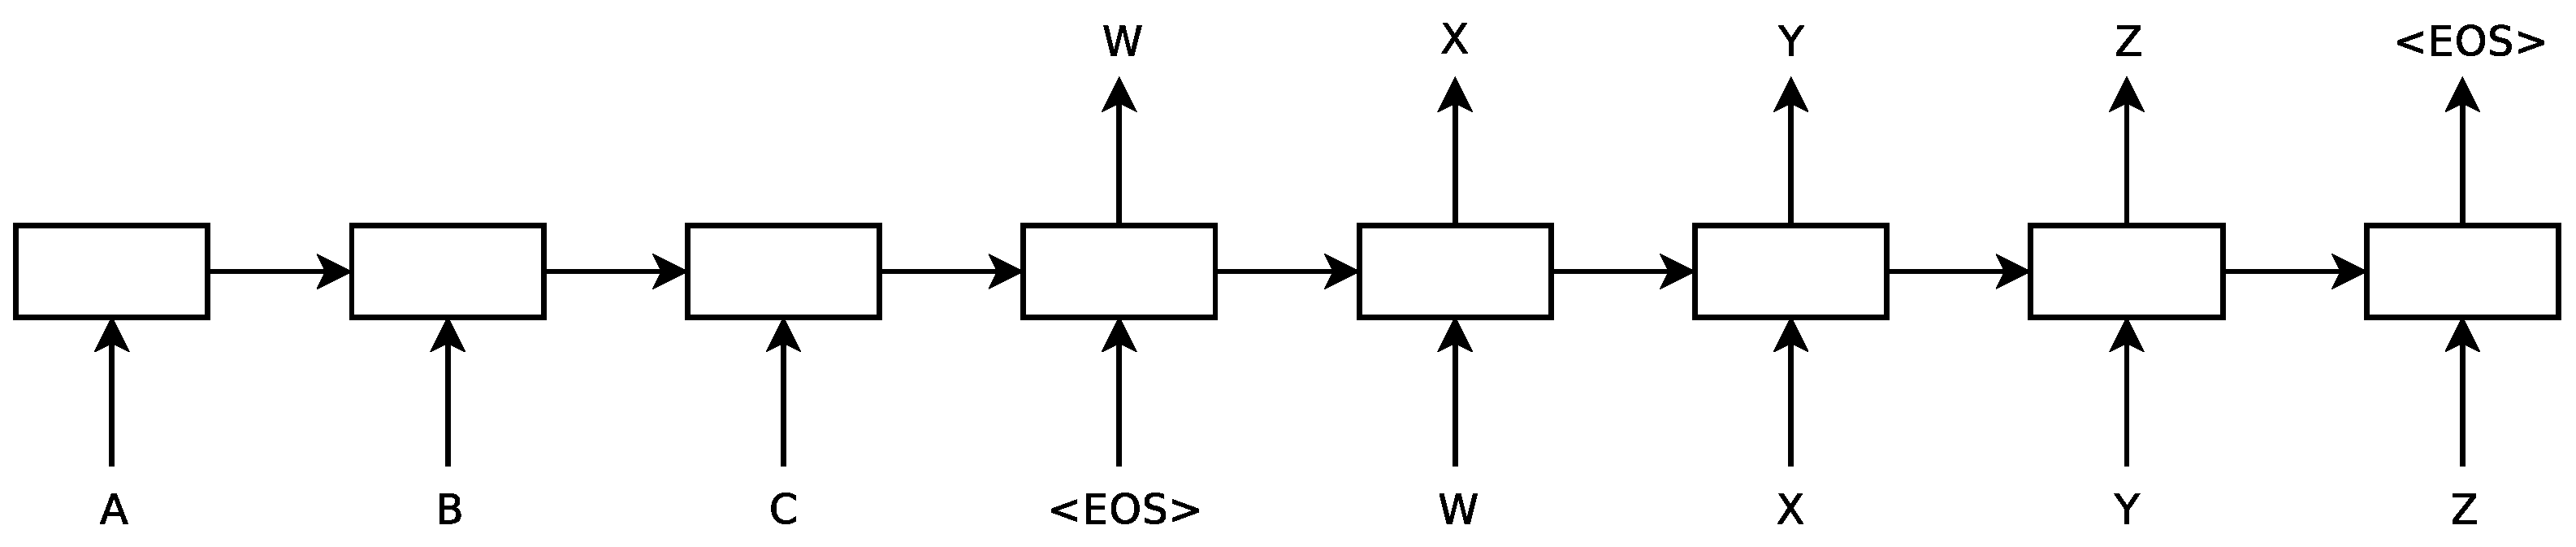
\includegraphics[width=0.9\textwidth]{Diagram1.eps}
\caption{\small 我们的模型读取输入句子“ABC”,并产生“WXYZ”作为输出句子。 该模型在输出句尾标记之后停止进行预测。 请注意,LSTM反向读取输入句子,因为这样做会在数据中引入许多短期依赖性,使得优化问题更容易。 }
\label{fig:translation-model2}
\end{figure}

这项工作的主要结果如下。在WMT'14将英语翻译成法语的任务中,我们通过使用简单的从左到右的束搜索解码直接从5个深LSTM的集合(每个具有380M个参数)中提取翻译,获得{\bf 34.81}的BLEU得分。这是迄今为止通过使用大型神经网络直接翻译所获得的最佳结果。为了比较,该数据集上的SMT基线的BLEU得分为33.30\cite{wmt14_en_fr}。通过LSTM实现的34.81 BLEU分数,词汇为80k字,所以当参考翻译包含这80k字以外的单词时,分数将被惩罚。这个结果表明比基于成熟短语的SMT系统表现更好的相对未优化的神经网络结构还具有很大的改进空间。

最后我们使用LSTM重新计算相同任务的SMT基准的1000个公开最好的列表得分\cite{wmt14_en_fr}。通过这样做,我们获得了36.5的BLEU得分,这提高了基线3.2个BLEU点,并接近以前发表过的最先进的水平(这是37.0\cite{durrani-EtAl:2014:W14-33})。

令人惊讶的是,LSTM没有遭受长句子的困扰,尽管其他研究者用相关的模型的经验表明可能会受到长句子的困扰\cite{curse}。我们能够在长句子上做得很好是因为我们颠倒了输入语句中的单词顺序,而不颠倒训练和测试集中的输出句子。通过这样做,我们引入了许多短期依赖,使优化问题更简单(见第\ref{sec:model}和\ref{sec:rev_rev}节)。因此,随机梯度下降(SGD)可以学习对长句没有问题的LSTM。在源句子中逆转单词的顺序这个技巧是这项工作的关键技术贡献之一。

LSTM的一个有用的属性是它可以学习将可变长度的输入语句映射成固定维度的向量表示。鉴于翻译往往是源语句的释义,翻译目标鼓励LSTM捕捉到其意义的句子表示,因为具有类似意义的句子彼此接近,而不同的句子意义将是远的。一个定性的评价支持表明我们的模型懂得词序,对于主动和被动语态是保持不变的。



\section{模型}
\label{sec:model}

循环神经网络(RNN)\cite{werbos,rumelhart1986learning}是序列的前馈神经网络的自然泛化。给定输入序列$(x_1,\ldots,x_T)$,一个标准的RNN通过迭代计算输出序列$(y_1,\ldots,y_T)$算式如下:
\begin{eqnarray*}
	h_t &=& \mathrm{sigm}\left(W^{\mathrm{hx}} x_t + W^{\mathrm{hh}} h_{t-1}\right) \\
	y_t &=& W^{\mathrm{yh}}h_t
\end{eqnarray*}
只要提前知道输入和输出之间的对齐,RNN很简单就能将输入映射到输出上。然而不清楚如何将RNN应用于其输入和输出序列具有不同长度的复杂和变化的问题。

一般序列学习的简单策略是使用一个RNN将输入序列映射到固定大小的向量,然后用另一个RNN将固定向量映射到输出序列((Cho等人\cite{cho14}也采用了这种方法)。虽然原则上它可以工作,但因为RNN提供了所有的相关信息并且存在长期依赖性,所以RNN难以训练(figure \ref{fig:translation-model2})
\cite{hochreiter_long_term,bengio_long_term,hochreiter97,Hochreiter01gradientflow}。然而,已知长短期记忆神经网络(LSTM)\cite{hochreiter97}可以在学习中解决长时间依赖性的问题,因此LSTM在这一设定下会成功。

LSTM的目标是估计条件概率$p(y_1,\ldots,y_{T'} | x_1,\ldots,x_T)$,其中$(x_1,\ldots,x_T)$是输入序列,$y_1,\ldots,y_{T'}$是对应的输出序列并且长度$T'$可能不等于$T$,LSTM先通过最后一个隐藏层获得$(x_1,\ldots,x_T)$的固定维度的表示$v$来计算这一条件概率,然后用一个初始隐藏状态设置为$v$的标准LSTM-LM公式来计算$y_1,\ldots,y_{T'}$的概率:
\begin{equation}
p(y_1,\ldots,y_{T'} | x_1,\ldots,x_T) = \prod_{t=1}^{T'} p(y_t | v, y_1, \ldots, y_{t-1})
\label{eqn:keyequation}
\end{equation}
在该等式中,每一个$p(y_t | v, y_1, \ldots, y_{t-1})$的分布用词汇表中所有单词进行的softmax来表示,我们使用Graves的LSTM公式\cite{graves13c}。我们要求每个句子以特殊的句尾符号``$<$EOS$>$''结束,这使得模型可以在任意长度的序列上来定义分布。总体的方法在图\ref{fig:translation-model2}中概述,其中表示的LSTM计算了``A'', ``B'', ``C'',``$<$EOS$>$''的表示,然后使用该表示来计算``W'',
``X'', ``Y'', ``Z'', ``$<$EOS$>$''的概率。

我们的实际模型有三个重要的方面不同于上面的描述。首先,我们使用两个不同的LSTM:一个用于输入序列,另一个用于输出序列,这样做可以以可忽略的计算成本增加模型参数的数量,并且非常自然地可以在多语言对上同时训练LSTM\cite{kal13}。第二,我们发现深层LSTM显着优于浅层LSTM,所以我们选择了一个有四层的LSTM。第三,我们发现扭转输入句子的顺序是非常有价值的。举个例子,不是将句子$a,b,c$映射到句子$\alpha,\beta,\gamma$,而是训练LSTM将$c,b,a$映射到$\alpha,\beta,\gamma$,其中$\alpha,\beta,\gamma$是$a,b,c$的翻译。这种方法使得$a$很接近$\alpha$,$b$很接近$\beta$,以此类推,这使得SGD容易在输入和输出之间“建立通信”。我们发现这个简单的数据转换大大提高了LSTM的性能。

%% It may appear that the LSTM is incapable of translating long sentences
%% \cite{bog14,curse,cho14}, which was also confirmed by our early
%% experiments.  We tried to address this problem by partitioning long
%% sentences into a small number of medium-sized pieces (of length 30)
%% and concatenate translations of each piece.  However, we found that
%% LSTMs trained on reversed source sentences were hurt by this technique
%% because could translate long sentences with little difficulty (see
%% fig.~\ref{fig:oriol}).




\section{实验}
\label{sec:experiments}
 
我们用了两种方法将我们的方法应用于WMT'14英语到法语机器翻译(MT)任务中。 我们使用它直接翻译输入句子而不参考统计机器翻译(SMT)系统,我们使用它来重新定义SMT基准的n个最佳列表。我们报告这些翻译方法的准确性,
呈现示例翻译,并可视化所得到的句子结果。

\subsection{Dataset details}

We used the WMT'14 English to French dataset.  We trained our models
on a subset of 12M sentences consisting of 348M French words and 304M
English words, which is a clean ``selected'' subset from
\cite{wmt14_en_fr}. We chose this translation task and this specific
training set subset because of the public availability of a tokenized training and
test set together with 1000-best lists from the baseline SMT 
\cite{wmt14_en_fr}.

As typical neural language models rely on a vector representation for
each word, we used a fixed vocabulary for both languages.  We used
160,000 of the most frequent words for the source language and 80,000
of the most frequent words for the target language.  Every
out-of-vocabulary word was replaced with a special ``UNK'' token.  
 
%% \subsection{Sentence-level Autoencoder}

%% To solve our translation task, the LSTM must store the entire input
%% sentence in its memory, and it is not clear that an LSTM can learn to
%% store the necessary amount of information in its hidden state.  Thus,
%% we start with the easier problem of memorizing an input sentence by
%% reading it into the hidden state and then outputting the same
%% sentence.  If this autoencoding task proves to be too difficult for
%% the LSTM, it would mean that our approach is relatively hopeless.

%% Luckily, we found that the LSTM could easily solve the memorization
%% problem, as it has achieved a perplexity of $1.03$ on the test set.
%% This very low perplexity suggests that at minimum, the LSTM is capable
%% of learning to store a sequence of words of an unknown length in a
%% vector of a fixed dimensionality.


\subsection{Decoding and Rescoring}

The core of our experiments involved training a large deep LSTM on
many sentence pairs. We trained it by maximizing the log
probability of a correct translation $T$ given the source sentence
$S$, so the training objective is
$$1/|\mathcal S|\sum_{(T,S)\in\mathcal S}\log p(T|S)$$ where $\mathcal
S$ is the training set.  Once training is complete, we produce
translations by finding the most likely translation according to
the LSTM:
\begin{equation}
\label{eqn:decode}
\hat{T} = \arg\max_T p(T|S)
\end{equation}
We search for the most likely translation using a simple left-to-right
beam search decoder which maintains a small number $B$ of partial
hypotheses, where a partial hypothesis is a prefix of some
translation.  At each timestep we extend each partial hypothesis in
the beam with every possible word in the vocabulary. This greatly
increases the number of the hypotheses so we discard all but the $B$
most likely hypotheses according to the model's log probability.  As soon
as the ``$<$EOS$>$'' symbol is appended to a hypothesis, it is removed from
the beam and is added to the set of complete hypotheses.  While this
decoder is approximate, it is simple to implement.  Interestingly, our
system performs well even with a beam size of 1, and a beam of
size 2 provides most of the benefits of beam search (Table
\ref{tab:blue_fr}).   

% todo:  insert note on removing very short solutions and solutions
% that consist entirely of the /UNK/ token. 

We also used the LSTM to rescore the 1000-best lists produced by the
baseline system \cite{wmt14_en_fr}.  To rescore an n-best list, we
computed the log probability of every hypothesis with our LSTM and
took an even average with their score and the LSTM's score.

\subsection{Reversing the Source Sentences}
\label{sec:rev_rev}

While the LSTM is capable of solving problems with long term
dependencies, we discovered that the LSTM learns much better when the
source sentences are reversed (the target sentences are not reversed).  By
doing so, the LSTM's test perplexity dropped from 5.8 to 4.7, and the 
test BLEU scores of its decoded translations increased from 25.9 to 30.6.



While we do not have a complete explanation to this phenomenon, we
believe that it is caused by the introduction of many short term
dependencies to the dataset.  Normally, when we concatenate a source
sentence with a target sentence, each word in the source sentence is
far from its corresponding word in the target sentence. As a result,
the problem has a large ``minimal time lag'' \cite{minimal_time_lag}.  By reversing the
words in the source sentence, the average distance between
corresponding words in the source and target language is unchanged.
However, the first few words in the source language are now very close to
the first few words in the target language, so the problem's minimal
time lag is greatly reduced. Thus, backpropagation has an easier time
``establishing communication'' between the source sentence and the
target sentence, which in turn results in substantially improved overall
 performance.

Initially, we believed that reversing the input sentences would 
only lead to more confident predictions in the early parts of the target
sentence and to less confident predictions in the later parts.
However, LSTMs trained on reversed source sentences did much better on
long sentences than LSTMs trained on the raw source sentences (see
sec.~\ref{sec:long_sentences}), which suggests that reversing the
input sentences results in LSTMs with better memory utilization. 



%% This result also suggests that hidden optimization issues are still
%% prevalent even in modern-day neural networks.  Prior to training LSTMs
%% on the reversed dataset, we believed that our models were
%% well-optimized, and that little could be gained with better
%% optimization methods.  However, the same architecture is clearly
%% capable of achieving much better results on essentially the same data, which
%% suggests that the worse performance of the ``forward'' LSTMs were entirely
%% due an optimization failure. 

%% \subsection{The Importance of Depth}

%% Deep LSTMs turned out to be important for MT tasks.  In earlier
%% experiments, we found that each additional layer reduced perplexity by
%% 10\%.  As we do not observe such perplexity reductions with deep LSTMs
%% on language modelling, it follows that most of the benefit of deep
%% LSTMs comes from their larger hidden state, which is important for our
%% formulation of MT where the hidden state needs to store the entire
%% input sentence.

\subsection{Training details}

We found that the LSTM models are fairly easy to train.  We used deep
LSTMs with 4 layers, with 1000 cells at each layer and 1000
dimensional word embeddings, with an input vocabulary of 160,000
and an output vocabulary of 80,000.  Thus the deep LSTM uses 8000 real 
numbers to represent a sentence. We found deep LSTMs to
significantly outperform shallow LSTMs, where each additional layer
reduced perplexity by nearly 10\%, possibly due to their much larger
hidden state.  We used a naive softmax over 80,000 words at each
output.  The resulting LSTM has 384M parameters of which 64M are pure
recurrent connections (32M for the ``encoder'' LSTM and 32M for the
``decoder'' LSTM). The complete training details are given below:
\begin{itemize}
\item We initialized all of the LSTM's parameters with the uniform distribution between
  -0.08 and 0.08
\item We used stochastic gradient descent without momentum,
  with a fixed learning rate of 0.7.  After 5 epochs, we begun
  halving the learning rate every half epoch.  We trained our models for a
  total of 7.5 epochs.
\item We used batches of 128 sequences for the gradient and divided it
  the size of the batch (namely, 128).
\item Although LSTMs tend to not suffer from the vanishing gradient
  problem, they can have exploding gradients.  Thus we enforced a hard
  constraint on the norm of the gradient
  \cite{graves13c,razvan} by scaling it when its norm exceeded
  a threshold. For each training batch, we compute $s =
  \left\|g\right\|_2$, where $g$ is the gradient divided by 128. If $s > 5$, we set
  $g = \frac{5g}{s}$.
\item Different sentences have different lengths.  Most sentences are
  short (e.g., length 20-30) but some sentences are long (e.g., length
  $>$ 100), so a minibatch of 128 randomly chosen training sentences
  will have many short sentences and few long sentences, and as a
  result, much of the computation in the minibatch is wasted.  To
  address this problem, we made sure that all sentences in a
  minibatch are roughly of the same length, yielding a 2x speedup.
\end{itemize}


\subsection{Parallelization}

A C++ implementation of deep LSTM with the configuration from the
previous section on a single GPU processes a speed of approximately
1,700 words per second.  This was too slow for our purposes, so we 
parallelized our model using an 8-GPU machine.  Each layer of the LSTM
was executed on a different GPU and communicated its activations
to the next GPU / layer as soon as they were computed.  Our models
have 4 layers of LSTMs, each of which resides on a separate GPU.  The remaining
4 GPUs were used to parallelize the softmax, so each GPU was
responsible for multiplying by a $1000\times 20000$ matrix.  The
resulting implementation achieved a speed of 6,300 (both English and
French) words per second with a minibatch size of 128. 
Training took about a ten days with this implementation.


\subsection{Experimental Results}

We used the cased BLEU score \cite{bleu} to evaluate the quality of our
translations. We computed our BLEU scores using \texttt{multi-bleu.pl}\footnote{
There several variants of the BLEU score, and each variant is defined  with a perl script. } 
on the \emph{tokenized} predictions and ground truth.
This way of evaluating the BELU score is consistent with \cite{cho14} and \cite{bog14}, and reproduces
the 33.3 score of \cite{wmt14_en_fr}.
However, if we evaluate the best WMT'14 system \cite{durrani-EtAl:2014:W14-33}
(whose predictions can be downloaded from \url{statmt.org\matrix}) in this manner, we get   
37.0, which is greater than the 35.8 reported by \url{statmt.org\matrix}.  

%% According to , 
%% the performance of the best English to French system on the WMT'14 \cite{durrani-EtAl:2014:W14-33}
%% is 35.8.  This score is obtained if we use the \texttt{mteval.pl} script on the \emph{untokenized}
%% test set.  We obtain 37.0 if we download the predictions of the best system from 
%% \url{statmt.org\matrix} and use \texttt{multi-bleu.pl} on the \emph{tokenized}
%% predictions.  This is done to be consistent with \cite{cho14} and \cite{bog14}.
%% All our scores 



%% We verified the correctness of our BLEU score
%% computation by reproducing the BLEU score of LIUM's baseline system using
%% its n-best list. Of particular importance were issues relating to
%% tokenization and normalization of the test sentences.  We made sure to ``unnormalize'' our
%% translations (for example, to replace ``they 're'' with ``they're''),
%% in order to reproducing the baseline's BLEU score with our
%% evaluation tools.

The results are presented in tables \ref{tab:blue_fr} and
\ref{tab:blue_fr_rescore}.  Our best results are obtained with an
ensemble of LSTMs that differ in their random initializations and
in the random order of minibatches.  While the decoded translations of the
LSTM ensemble do not outperform the best WMT'14 system, it is the first time
that a pure neural translation system outperforms a 
phrase-based SMT baseline on a large scale MT task by a sizeable margin,
despite its inability to handle out-of-vocabulary words.  The LSTM
is within 0.5 BLEU points of the best WMT'14 result if it is used to rescore the 1000-best
list of the baseline system.

\begin{table}[t]
\centering
\begin{small}
\begin{tabular}{|c|c|}
\hline
{\bf Method}  & {\bf test BLEU score (ntst14) } \\ \hline
Bahdanau et al. \cite{bog14}  &  28.45 \\ \hline
Baseline System  \cite{wmt14_en_fr} & 33.30 \\ \hline
\hline
Single forward LSTM, beam size 12 & 26.17 \\ \hline                 
Single reversed LSTM, beam size 12 & 30.59 \\ \hline
Ensemble of 5 reversed LSTMs, beam size 1  &  33.00 \\ \hline
Ensemble of 2 reversed LSTMs, beam size 12  &  33.27 \\ \hline
Ensemble of 5 reversed LSTMs, beam size 2  &  34.50 \\ \hline
Ensemble of 5 reversed LSTMs, beam size 12  &  {\bf 34.81} \\ \hline
\end{tabular}
\end{small}
\caption{The performance of the LSTM on WMT'14 English to French test
  set (ntst14).  Note that an ensemble of 5 LSTMs with a beam of size
  2 is cheaper than of a single LSTM with a beam of size 12.  }
\label{tab:blue_fr}
\end{table}

\begin{table}[]
\centering
\begin{small}
\begin{tabular}{|c|c|}
\hline
{\bf Method}  & {\bf test BLEU score (ntst14) } \\ \hline
Baseline System  \cite{wmt14_en_fr} & 33.30 \\ \hline
Cho et al. \cite{cho14}  & 34.54 \\ \hline 
Best WMT'14 result \cite{durrani-EtAl:2014:W14-33} &  {\bf 37.0} \\ \hline
\hline
Rescoring the baseline 1000-best with a single forward LSTM & 35.61 \\ \hline 
Rescoring the baseline 1000-best with a single reversed  LSTM & 35.85 \\ \hline  %wmt_FREN_good_rescore_80k_one_rev_1.merge
%Rescoring the LIUM 1000-best with 5 forward LSTMs  &  36.3 \\ \hline    
Rescoring the baseline 1000-best with an ensemble of 5 reversed LSTMs  &  {\bf 36.5} \\ \hline    %wmt_FREN_good_rescore_80k_all_rev_1.merge 
\hline
Oracle Rescoring of the Baseline 1000-best lists    & $\sim$45 \\ \hline 
\end{tabular}
\end{small}
\caption{Methods that use neural networks together with an SMT system
  on the WMT'14 English to French test set (ntst14).}
\label{tab:blue_fr_rescore}
\end{table}



\subsection{Performance on long sentences}
\label{sec:long_sentences}

We were surprised to discover that the LSTM did well on long
sentences, which is shown quantitatively in figure \ref{fig:oriol}.
Table \ref{tab:examples} presents several examples of long sentences and
their translations. 

\begin{table}[ht!]
\centering
\begin{footnotesize}
\begin{tabular}{|l|l|}
\hline
{\bf  Type} & {\bf Sentence} \\ 
\hline
\hline
{\bf Our model} & Ulrich UNK , membre du conseil d' administration du constructeur automobile Audi , \\
& affirme qu' il s' agit d' une pratique courante depuis des ann\'{e}es pour que les t\'{e}l\'{e}phones \\
& portables  puissent  \^{e}tre collect\'{e}s avant les r\'{e}unions du conseil d' administration afin qu' ils\\
&  ne soient pas  utilis\'{e}s comme appareils d' \'{e}coute \`{a} distance .\\
%%Ulrich UNK , membre du conseil d'administration du constructeur automobile Audi  \\
%%&  , affirme qu'il les r\'{e}unions du s'agit d'une pratique  courante depuis des ann\'{e}es pour      \\
%%& que les t\'{e}l\'{e}phones portables puissent \^{e}tre collect\'{e}s avant conseil d'administration afin     \\
%%& qu'ils ne soient pas utilis\'{e}s comme appareils d'\'{e}coute \`{a} distance . \\
%\hline
%{\bf EN} & UNK Ulrich, a member of the board of automaker Audi says that this is a common  \\
%{\bf LSTM}& practice for years that mobile phones can be collected before the meetings of the board so that  \\
%& they do are not used as remote listening devices. \\
\hline
{\bf  Truth} &  Ulrich Hackenberg , membre du conseil d' administration du constructeur automobile Audi ,   \\
& d\'{e}clare que la collecte des t\'{e}l\'{e}phones portables avant les r\'{e}unions du conseil , afin qu' ils  \\
& ne puissent pas \^{e}tre utilis\'{e}s comme appareils d' \'{e}coute \`{a} distance , est une pratique courante \\ 
& depuis des ann\'{e}es .\\
\hline\hline
%{\bf EN} &  Ulrich Hackenberg, member of the board of automaker Audi said that the  \\
%{\bf Truth} & collection of mobile phones before board meetings, so they can not be used as listening devices  \\
%& remotely, is a common practice for years.\\
{\bf Our model} & 
`` Les t\'{e}l\'{e}phones cellulaires , qui sont vraiment une question , non seulement parce qu' ils \\
& pourraient potentiellement causer des interf\'{e}rences avec les appareils de navigation , mais \\
& nous savons , selon la FCC , qu' ils pourraient interf\'{e}rer avec les tours de t\'{e}l\'{e}phone cellulaire \\
& lorsqu' ils sont dans l' air '' , dit UNK .\\
%%``Les t\'{e}l\'{e}phones cellulaires , qui sont vraiment une question , non seulement parce \\
%%& qu'ils pourraient potentiellement causer des interf\'{e}rences avec les appareils de navigation , \\
%%& mais nous savons , selon la FCC , qu'ils pourraient interf\'{e}rer avec les tours de t\'{e}l\'{e}phone cellulaire \\
%%&  lorsqu'ils sont dans l'air `` , dit UNK .  \\
\hline
{\bf Truth} & 
`` Les t\'{e}l\'{e}phones portables sont v\'{e}ritablement un probl\`{e}me , non seulement parce qu' ils \\
& pourraient \'{e}ventuellement cr\'{e}er des interf\'{e}rences avec les instruments de navigation , mais \\
& parce que nous savons , d' apr\`{e}s la FCC , qu' ils pourraient perturber les antennes-relais de \\
& t\'{e}l\'{e}phonie mobile s' ils sont utilis\'{e}s \`{a} bord '' , a d\'{e}clar\'{e} Rosenker .\\
%%`` Les t\'{e}l\'{e}phones portables sont v\'{e}ritablement un probl\'{e}me , non seulement parce qu'ils \\
%%& pourraient \'{e}ventuellement cr\'{e}er des interf\'{e}rences avec les instruments de navigation , mais parce \\
%%& que nous savons , d'apr\`{e}s la FCC , qu'ils pourraient perturber les antennes-relais de \\
%%& t\'{e}l\'{e}phonie mobile s'ils sont utilis\'{e}s \`{a} bord '' , a d\'{e}clar\'{e} Rosenker . \\
\hline\hline
{\bf Our model} & 
Avec la cr\'{e}mation , il y a un `` sentiment de violence contre le corps d' un \^{e}tre cher '' , \\
& qui sera `` r\'{e}duit \`{a} une pile de cendres '' en tr\`{e}s peu de temps au lieu d' un processus de \\
& d\'{e}composition ``  qui accompagnera les \'{e}tapes du deuil '' .\\
%%Avec la cr\'{e}mation , il y a un `` sentiment de violence contre le corps d'un \^{e}tre cher `` , \\ 
%%& qui sera `` r\'{e}duit \`{a} une pile de cendres `` en tr\`{e}s peu de temps au lieu d'un processus de d\'{e}composition \\
%%&  `` qui accompagnera les \'{e}tapes du deuil `` . \\  
\hline
{\bf Truth} & 
Il y a , avec la cr\'{e}mation , `` une violence faite au corps aim\'{e} '' , \\
& qui va \^{e}tre `` r\'{e}duit \`{a} un tas de cendres '' en tr\`{e}s peu de temps , et non apr\`{e}s un processus de \\
&d\'{e}composition , qui `` accompagnerait les phases du deuil '' .\\
%%Il y a , avec la cr\'{e}mation , `` une violence faite au corps aim\'{e} `` , qui va \^{e}tre `` r\'{e}duit \\
%%&  \`{a} un tas de cendres `` en tr\`{e}s peu de temps , et non apr\`{e}s un processus de d\'{e}composition , qui `` \\
%%&accompagnerait les phases du deuil `` .\\
\hline
\end{tabular}
\end{footnotesize}
\caption{A few examples of long translations produced by the LSTM
  alongside the ground truth translations.  The reader can verify that
  the translations are sensible using Google translate.  }
\label{tab:examples}
\end{table}



%% \begin{table}[ht!]
%% \centering
%% \begin{footnotesize}
%% \begin{tabular}{|l|l|}
%% \hline
%% {\bf  Type} & {\bf Sentence} \\ 
%% \hline
%% {\bf LSTM} & Ulrich UNK , membre du conseil d'administration du constructeur automobile Audi  \\
%% &  , affirme qu'il les réunions du s'agit d'une pratique  courante depuis des années pour      \\
%% & que les téléphones portables puissent être collectés avant conseil d'administration afin   	  \\
%% & qu'ils ne soient pas utilisés comme appareils d'écoute à distance . \\
%% %\hline
%% %{\bf EN} & UNK Ulrich, a member of the board of automaker Audi says that this is a common  \\
%% %{\bf LSTM}& practice for years that mobile phones can be collected before the meetings of the board so that  \\
%% %& they do are not used as remote listening devices. \\
%% \hline
%% {\bf  Truth} &  Ulrich Hackenberg , membre du conseil d'administration du constructeur    \\
%% & automobile Audi , déclare que la des téléphones portables avant les réunions du conseil , afin qu'ils  \\
%% & ne puissent pas être utilisés comme appareils collecte d'écoute à distance ,  \\
%% &  est une pratique courante depuis des années . \\
%% \hline\hline
%% %{\bf EN} &  Ulrich Hackenberg, member of the board of automaker Audi said that the  \\
%% %{\bf Truth} & collection of mobile phones before board meetings, so they can not be used as listening devices  \\
%% %& remotely, is a common practice for years.\\
%% {\bf LSTM} & ``Les téléphones cellulaires , qui sont vraiment une question , non seulement parce \\
%% & qu'ils pourraient potentiellement causer des interférences avec les appareils de navigation , \\
%% & mais nous savons , selon la FCC , qu'ils pourraient interférer avec les tours de téléphone cellulaire \\
%% &  lorsqu'ils sont dans l'air `` , dit UNK .  \\
%% \hline
%% {\bf Truth} & `` Les téléphones portables sont véritablement un problème , non seulement parce qu'ils \\
%% & pourraient éventuellement créer des interférences avec les instruments de navigation , mais parce \\
%% & que nous savons , d'après la FCC , qu'ils pourraient perturber les antennes-relais de \\
%% & téléphonie mobile s'ils sont utilisés à bord '' , a déclaré Rosenker . \\
%% \hline\hline
%% {\bf LSTM} & Avec la crémation , il y a un `` sentiment de violence contre le corps d'un être cher `` , \\ 
%% & qui sera `` réduit à une pile de cendres `` en très peu de temps au lieu d'un processus de décomposition \\
%% &  `` qui accompagnera les étapes du deuil `` . \\  
%% \hline
%% {\bf Truth} & Il y a , avec la crémation , `` une violence faite au corps aimé `` , qui va être `` réduit \\
%% &  à un tas de cendres `` en très peu de temps , et non après un processus de décomposition , qui `` \\
%% &accompagnerait les phases du deuil `` .\\
%% \hline
%% \end{tabular}
%% \end{footnotesize}
%% \caption{The table shows a few examples of long translations produced
%%   by the LSTM together with the ground truth translations.  The reader
%%   can verify using Google translate that the LSTM's translations are  
%%   basically correct.
%%  }
%% \label{tab:examples}
%% \end{table}


\subsection{Model Analysis}

\begin{figure}[h!]
\centering
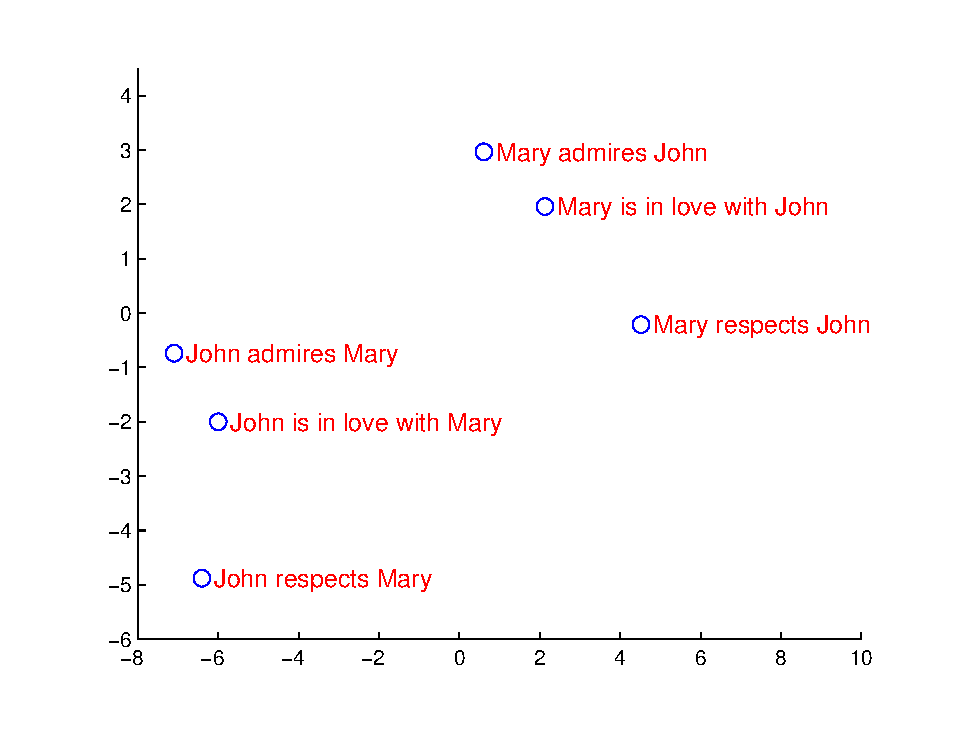
\includegraphics[width=0.46\textwidth]{figure2} ~~
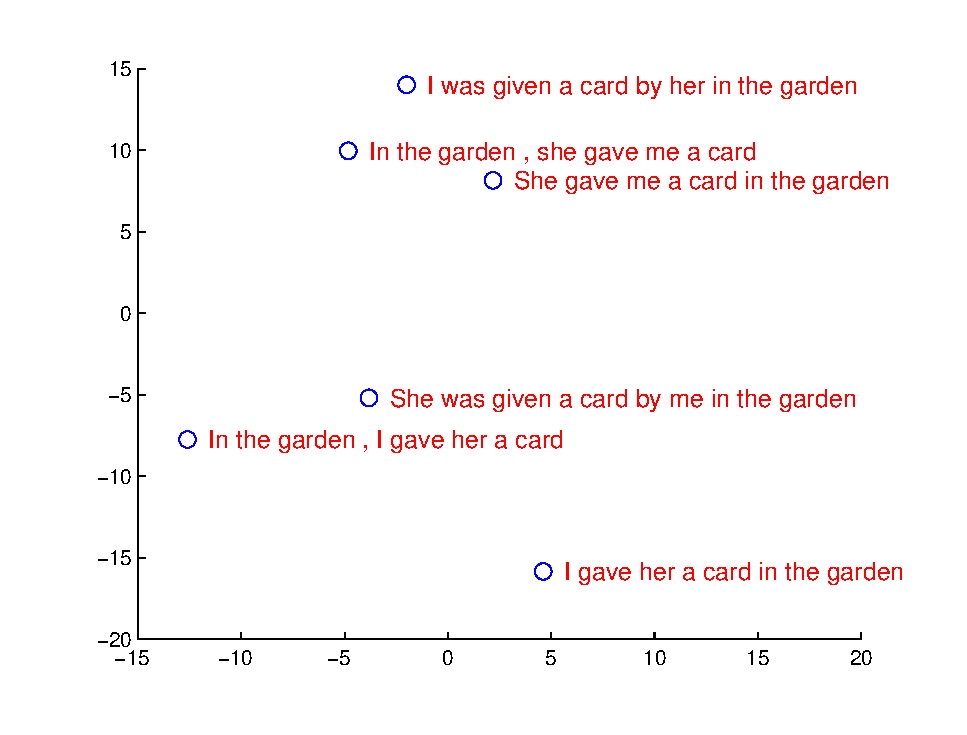
\includegraphics[width=0.46\textwidth]{figure3} 
\caption{\small The figure shows a 2-dimensional PCA projection of the
  LSTM hidden states that are obtained after processing the phrases in
  the figures.  The phrases are clustered by meaning, which in these
  examples is primarily a function of word order, which would be
  difficult to capture with a bag-of-words model. Notice that both
  clusters have similar internal structure.}
\label{fig:embedding}
\end{figure}

%good1} }
\begin{figure}[h!]
\centerline{
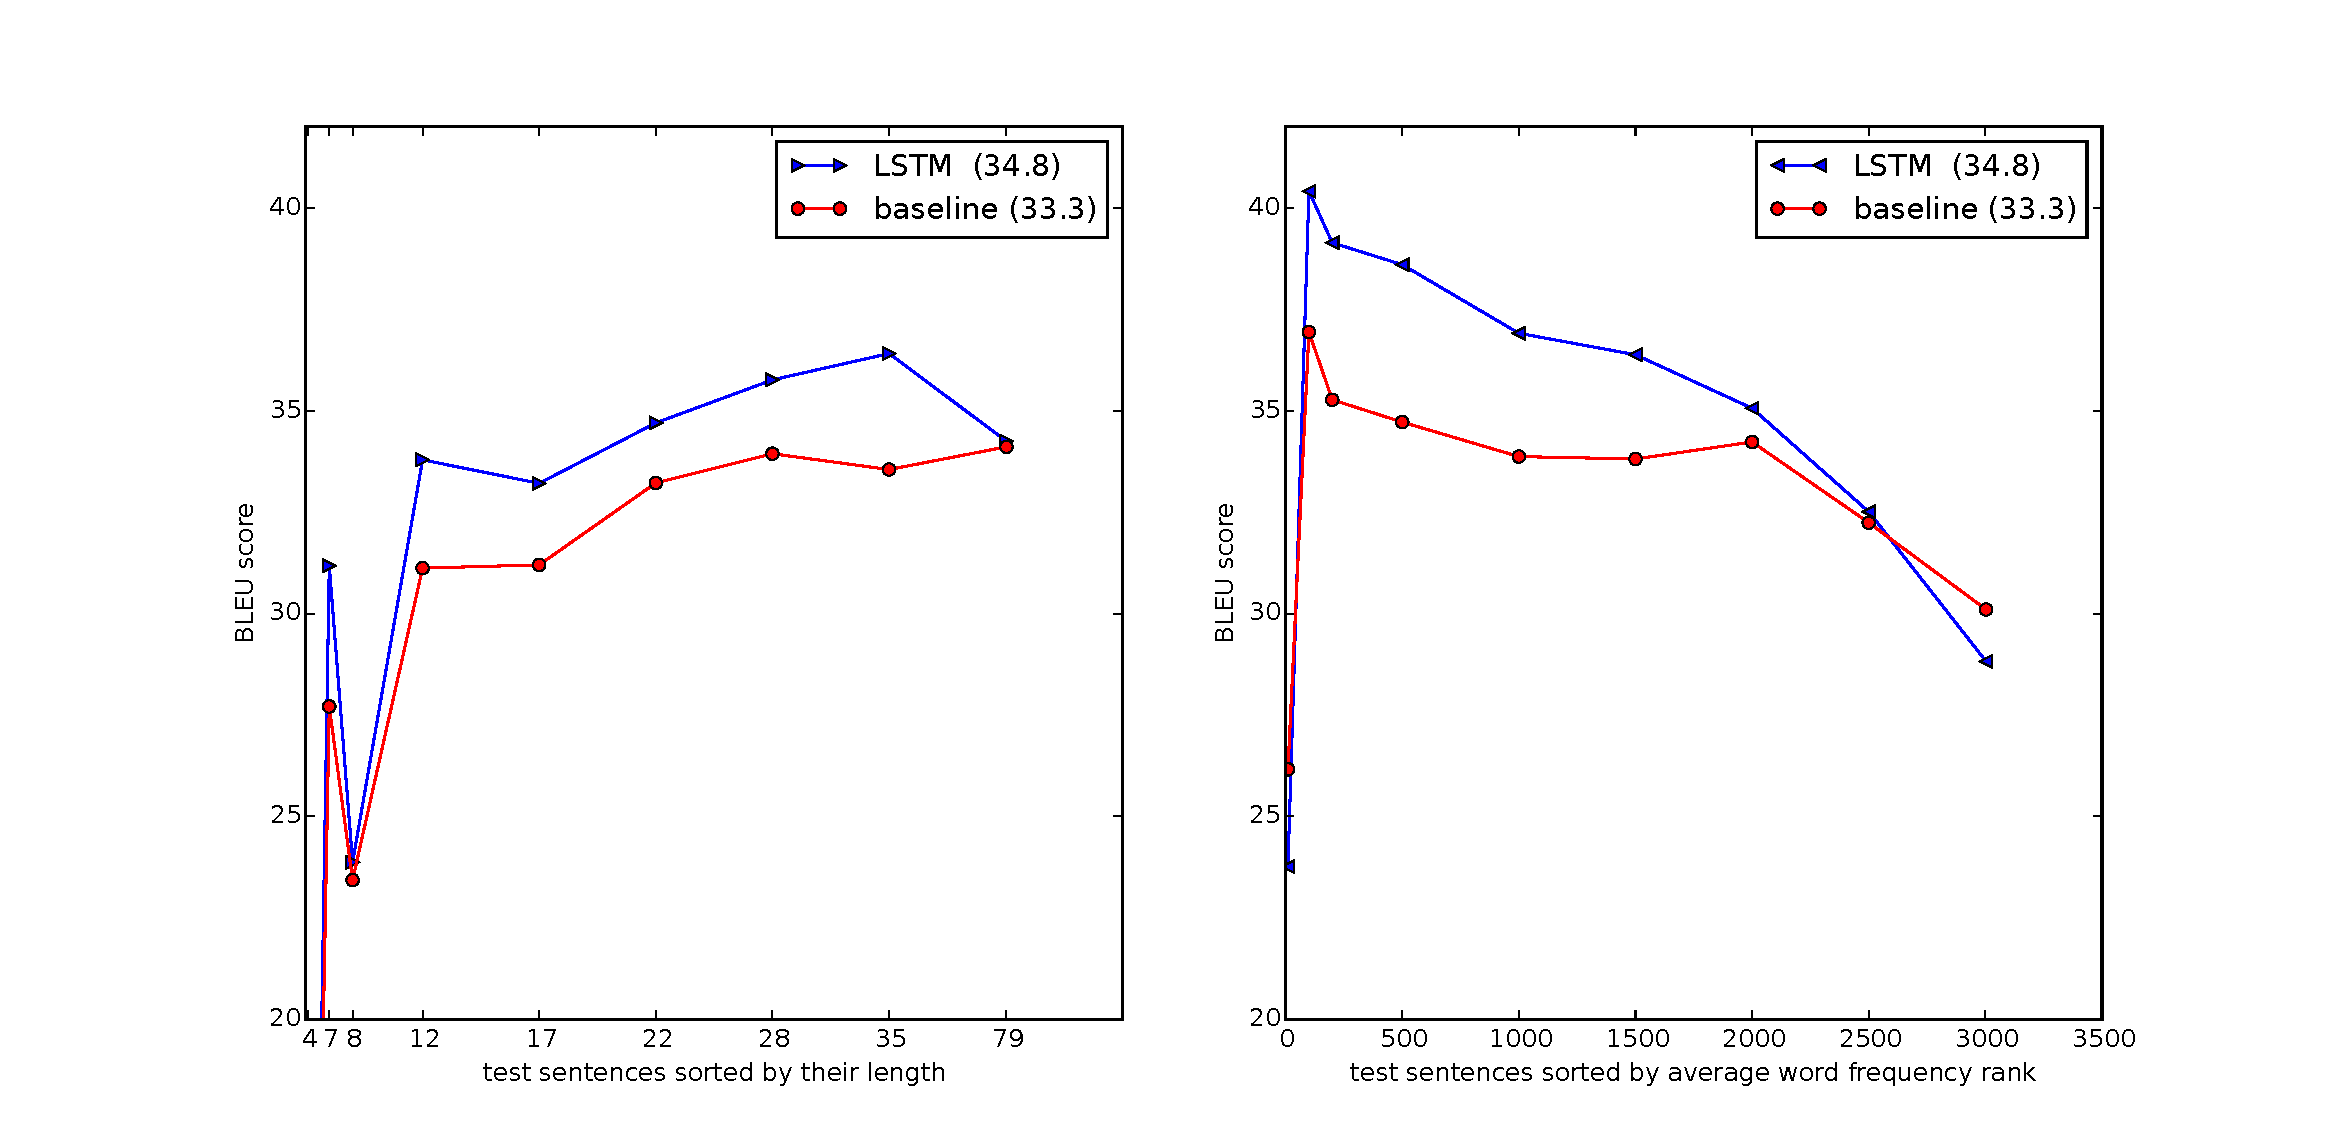
\includegraphics[width=1.\textwidth]{good2.eps} }  
\caption{\small The left plot shows the performance of our system as a
  function of sentence length, where the x-axis corresponds to the
  test sentences sorted by their length and is marked by the actual
  sequence lengths.  There is no degradation on sentences with less
  than 35 words, there is only a minor degradation on the longest
  sentences.  The right plot shows the LSTM's performance on sentences
  with progressively more rare words, where the x-axis corresponds to
  the test sentences sorted by their ``average word frequency rank''.
}
\label{fig:oriol}
\end{figure}

%% In our experiments, we trained LSTMs with only 4 layers, but deeper
%% LSTMs would achieve even better translation performance, every
%% additional LSTM layer reduced the perplexity by almost 10\%.  It is
%% easy to see why it should be so: the deeper LSTMs have much more
%% hidden state, so they have an easier time storing the input sequence.

One of the attractive features of our model is its ability to turn a
sequence of words into a vector of fixed dimensionality.
Figure~\ref{fig:embedding} visualizes some of the learned
representations.  The figure clearly shows that the representations
are sensitive to the order of words, while being fairly insensitive to
the replacement of an active voice with a passive voice.  The
two-dimensional projections are obtained using PCA.








\section{相关工作}
\label{sec:rel_work}

有大量的神经网络应用于机器翻译的工作。到目前为止,将RNN语言模型(RNNLM)\cite{mikolov2010recurrent}或前馈神经网络语言模型(NNLM)\cite{bengio}应用于机器翻译任务的最简单和最有效的方法是通过重新计算机器翻译基线的最优列表\cite{mikolov2012},可以可靠地提高翻译质量。

最近,研究人员已经开始研究如何在NNLM中包含源语言的信息,这项工作的例子包括Auli等人\cite{auli13},他们结合NNLM与输入句子的主题模型,这提高了重新评分的表现。Devlin等人\cite{devlin14}遵循类似的方法,但他们将他们的NNLM合并到机器翻译系统的解码器,并使用解码器的对齐信息为NNLM提供输入句子中最有用的词。他们的方法非常成功并且在基准上取得了很大的改进。

我们的工作与Kalchbrenner和Blunsom\cite{kal13}密切相关,他们是第一个将输入句子映射到一个向量然后回到一个句子的人,虽然他们使用卷积神经网络将句子映射到向量,这丢失了单词的排序
。类似于这项工作,Cho等人\cite{cho14}使用类似LSTM的RNN架构将句子映射到向量再返回到句子,他们的主要焦点是将神经网络集成到SMT系统。Bahdanau等人\cite{bog14}也试图用神经网络直接翻译并且使用了注意机制克服Cho等人\cite{cho14}长句子上的不良表现并取得了令人鼓舞的成果。同样,Pouget-Abadie等人\cite{curse}试图解决Cho等人\cite{cho14}的记忆问题,他们通过翻译源语句的片段来获得平滑的翻译,这类似于基于短语的方法。我们怀疑他们可以在训练神经网络时通过反向源句子来实现类似的改进。


端对端训练也是Hermann等人\cite{hermann14}的焦点,其模型表示前馈网络的输入和输出,并将它们映射到空间中的类似点。然而他们的方法不能直接生成翻译:为了得到翻译,他们需要在预先计算的句子数据库中查找最接近的向量,或者重新定义句子。


\section{结论}

在这项工作中,我们展示了一个有限词汇量的大的深层LSTM表现胜过一个标准的基于SMT的系统,在大规模的MT任务中词汇可以是无限的。我们在机器翻译上的简单的基于LSTM的方法的成功表明,只要他们有足够的训练数据,它应该在许多其他序列学习问题上做得很好。

我们对通过翻转源语句中的词的顺序而获得的改进的程度感到惊讶。我们得出结论,找到一个具有最大数量的短期依赖问题编码是重要的,因为它们使学习问题更简单。特别地,尽管我们不能在非反向翻译问题(图\ref{fig:translation-model2}所示)上训练标准RNN,我们认为,当源语句颠倒时,标准的RNN应该很容易训练
(虽然我们没有通过实验验证)。

我们也对LSTM正确翻译很长句子的能力感到惊讶。我们最初相信LSTM将由于其有限的记忆会在长句子上失败,并且其他研究人员报告过与我们类似的模型在长句子上差的性能\cite{cho14,bog14,curse}。然而,对反转数据集上训练的LSTM在翻译长句子上没有什么困难。

最重要的是,我们展示了一个简单,直接和相对未优化的方法,这个方法可以超越成熟的SMT系统,因此进一步的工作可能会进一步提高翻译精度。这些结果表明,我们的方法可能在其他具有挑战的序列问题上表现很好。




\small
\section{Acknowledgments}

We thank Samy Bengio, Jeff Dean, Matthieu Devin, Geoffrey Hinton, Nal Kalchbrenner, Thang Luong, Wolfgang
Macherey, Rajat Monga, Vincent Vanhoucke, Peng Xu, Wojciech Zaremba,
and the Google Brain team for useful comments and discussions.


\bibliography{translate} 
\bibliographystyle{plain}
\end{document}
